\documentclass[onecolumn, draftclsnofoot,10pt, compsoc]{IEEEtran}
\usepackage{graphicx}
\usepackage{url}
\usepackage{setspace}
\usepackage{indentfirst}
\usepackage{longtable}
\usepackage{pdfpages}

\usepackage{geometry}
\geometry{textheight=9.5in, textwidth=7in}

% 1. Fill in these details
\def \CapstoneTeamName{		    The Apolloers}
\def \CapstoneTeamNumber{		49}
\def \GroupMemberOne{			Jonathan Ropp}
\def \GroupMemberTwo{			Shannon Sandy}
\def \GroupMemberThree{			Dean Akin}
\def \CapstoneProjectName{		Apollo 11 3D Animation}
\def \CapstoneSponsorCompany{	OMSI}
\def \CapstoneSponsorPersona{	Jim Todd}
\def \CapstoneSponsorPersonb{	Mike Bailey}

% 2. Uncomment the appropriate line below so that the document type works
\def \DocType{		
                %Problem Statement
				%Requirements Document Draft
				%Technology Review
				%Design Document
				%Progress Report
				Project Hand Off
				}
			
\newcommand{\NameSigPair}[1]{\par
\makebox[2.75in][r]{#1} \hfil 	\makebox[3.25in]{\makebox[2.25in]{\hrulefill} \hfill		\makebox[.75in]{\hrulefill}}
\par\vspace{-12pt} \textit{\tiny\noindent
\makebox[2.75in]{} \hfil		\makebox[3.25in]{\makebox[2.25in][r]{Signature} \hfill	\makebox[.75in][r]{Date}}}}
% 3. If the document is not to be signed, uncomment the RENEWcommand below
\renewcommand{\NameSigPair}[1]{#1}

%%%%%%%%%%%%%%%%%%%%%%%%%%%%%%%%%%%%%%%
\begin{document}
\begin{titlepage}
    \pagenumbering{gobble}
    \begin{singlespace}
        \hfill 
        % 4. If you have a logo, use this includegraphics command to put it on the coversheet.
        
\includegraphics[height=2cm]{OSU_horizontal_2C_O_over_B.eps}   
        \par\vspace{.2in}
        \centering
        \scshape{
            \huge CS Capstone \DocType \par
            {\large\today}\par
            \vspace{.5in}
            \textbf{\Huge\CapstoneProjectName}\par
            \vfill
            {\large Prepared for}\par
            \Huge \CapstoneSponsorCompany\par
            \vspace{5pt}
            {\Large\NameSigPair{\CapstoneSponsorPersona}\par}
            {\Large\NameSigPair{\CapstoneSponsorPersonb}\par}
            {\large Prepared by }\par
            Group\CapstoneTeamNumber\par
            % 5. comment out the line below this one if you do not wish to name your team
            \CapstoneTeamName\par 
            \vspace{5pt}
            {\Large
                \NameSigPair{\GroupMemberOne}\par
                \NameSigPair{\GroupMemberTwo}\par
                \NameSigPair{\GroupMemberThree}\par
            }
            \vspace{20pt}
        }
        \begin{abstract}
        % 6. Fill in your abstract   
    
We did a super awesome thing! 

        \end{abstract}     
    \end{singlespace}
\end{titlepage}
\newpage
\pagenumbering{arabic}
\tableofcontents

%%%%%%%%%%%%%%%%%%%%%%%%%%%%%%%%%%%%%%%%%%%%%%%%%%%%%%%%%%%%%%%%%%%%%%%%%
%%%%%%%%%%%%%%%%%%%%%%%%%%%%%%%%%%%%%%%%%%%%%%%%%%%%%%%%%%%%%%%%%%%%%%%%%
\section{Introduction to Project}

During the 2018-2019 school year, our team worked on creating a 3-D animation of the  Apollo 11 Moon Landing. Jim Todd, the planetarium director at the Oregon Museum of Science and Industry (OMSI) requested this project for Summer 2019, which will mark the 50th anniversary of the moon landing. Our goal was to accurately depict the Apollo 11 mission in a way that was historically accurate, as well as creating something that would be engaging for all audiences at OMSI, ranging from young children to astrology experts. 

Three Senior Computer Science Majors formed our team: Dean Akin, Jonathan Ropp, and Shannon Sandy. Mike Bailey, a computer graphics professor at Oregon State University, mentored our group, which was coined \textit{The Apolloers}. We all made progress on all aspects of the animation, but in general, Dean was in charge of keyframing and shaders, Jonathan focused on positioning and documentation, and Shannon compiled mission audio and the lunar surface. Additionally, we worked together on obtaining and loading objects, lighting, and more. Jim Todd also gave us guidance related to how things would realistically look while on the lunar surface. While we were only able to meet in person twice during this project, Jim always gave great feedback and gave us pointers to keep moving forward with the project. 

Who requested it?
Jim Todd, Director of Space Science Education at OMSI requested we make an animation about the Apollo 11 mission.
Why was it requested?
It was meant to be a commemoration of the feats that were achieved during the Apollo 11 mission. 
What is its importance?
It also will serve as a educational tool to teach about what we could achieve back then, and what we can achieve right now.
Who was/were your client(s)?
Jim Todd, Director of Space Education at OMSI, and Mike Bailey, Professor of Computer Science at Oregon State University.
Who are the members of your team?
Shannon Sandy, Jonathan Ropp, Dean A. Akin
What were their roles?
Dean did keyframe animation as well as lighting on the Earth and Moon. Shannon did work on the audio clips, as well as the landing animations. She created the feathered landing site zoom animation as well as work and improve on lighting shaders. Jonathan created the flight path in its entirety, formulated the bezier curves of the static path as well as the dynamic moving flight path through the use of the aformentioned keyframing animation class. 
What was the role of the client(s)? (I.e., did they supervise only, or did they participate in doing development)
We met with Jim Todd 2 times before, both times we were briefed on how the planetarium system worked as well as given examples of scripts written in their in-house scripting language, Dark-Matter. We use these scripts as references when we are transfering our project into a Dark-Matter native animation. Communication is limited due to distance and schedules, and because of this, Jim was not present during a majority of the development of the animation, but was present for all of the documentation and provided contextual information important to make the animation as authentic as possible. Dr. Bailey's involvement was day to day, and he was present during a majority of the development of the animation and documentation, and has even contributed a significant amount to the development of the project in the form of pertinent information, technical support, and code contribution. 
%%%%%%%%%%%%%%%%%%%%%%%%%%%%%%%%%%%%%%%%%%%%%%%%%%%%%%%%%%%%%%%%%%%%%%%%%
%%%%%%%%%%%%%%%%%%%%%%%%%%%%%%%%%%%%%%%%%%%%%%%%%%%%%%%%%%%%%%%%%%%%%%%%%
\section{Requirements doc}
\begin{titlepage}
    \pagenumbering{gobble}
    \begin{singlespace}
        \hfill 
        % 4. If you have a logo, use this includegraphics command to put it on the coversheet.
        
\includegraphics[height=2cm]{OSU_horizontal_2C_O_over_B.eps}   
        \par\vspace{.2in}
        \centering
        \scshape{
            \huge CS Capstone Requirements Document \par
            {\large\today}\par
            \vspace{.5in}
            \textbf{\Huge\CapstoneProjectName}\par
            \vfill
            {\large Prepared for}\par
            \Huge \CapstoneSponsorCompany\par
            \vspace{5pt}
            {\Large\NameSigPair{\CapstoneSponsorPersona}\par}
            {\large Prepared by }\par
            Group\CapstoneTeamNumber\par
            % 5. comment out the line below this one if you do not wish to name your team
            \CapstoneTeamName\par 
            \vspace{5pt}
            {\Large
                \NameSigPair{\GroupMemberOne}\par
                \NameSigPair{\GroupMemberTwo}\par
                \NameSigPair{\GroupMemberThree}\par
            }
            \vspace{20pt}
        }
        \begin{abstract}
        % 6. Fill in your abstract    
        	Our group, The Apolloers, is working with Mike Bailey to create a 3D animation about the Apollo 11 Moon Landing. This animation will be put on display in OMSI during the Summer of 2019 for the 50th anniversary of the Apollo 11 mission. The project will allow viewers to see what it is like on the Moon through animated views placed throughout the scene. This document breaks the project into requirements that we will use to guide our project through the development process. 
        \end{abstract}     
    \end{singlespace}
\end{titlepage}
\newpage
\pagenumbering{arabic}
%\tableofcontents
\subsection*{Revisions}
\begin{tabular} {|p{3.25cm}|p{5cm}|p{7cm}|}
\hline
Section & Original & New \\ \hline
1.2 - Scope & \begin{itemize}
  \item Animate entire mission
  \item 25 minutes
\end{itemize} & \begin{itemize}
  \item Focus on the Lunar Surface
  \item 10 minutes, allowing for questions
\end{itemize}\\ \hline
2.2 3.2 - Functions & \begin{itemize}
  \item Go through mission from launch to splashdown
\end{itemize} & \begin{itemize}
  \item Beginning and end with historic video, middle for interactive views
\end{itemize}\\ \hline
3.1 - External Interfaces & \begin{itemize}
  \item Unsure how to implement the animation at OMSI
\end{itemize} & \begin{itemize}
  \item The planetarium uses a unique script that we will translate our project into
\end{itemize}\\ \hline

\end{tabular}


% 7. uncomment this (if applicable). Consider adding a page break.
%\listoffigures
%\listoftables
\clearpage

% 8. now you write!
\subsection{Introduction}
Our group will be recreating the Apollo 11 mission using 3D graphics. This project is for the Oregon Museum of Science and Industry to display in their planetarium for the 50th anniversary of the Apollo 11 mission. This document contains the requirements for this project that our group and client, Jim Todd, have agreed upon. These requirements act as a definitive list of features that our project will need to implement in order for it to be considered complete. 
    \subsubsection{Purpose}
    The purpose of this project is to educate the general public about the Apollo 11 mission as well as to commemorate the mission's 50th anniversary. Our goal is to create the video so that the audience at OMSI will appreciate the complexity of the mission while also being entertained. 
    \subsubsection{Scope}
    This project will be an animation whose target audience are the people attending the planetarium at OMSI. This includes school children on a field trip, people interested in space travel, and people who are attending the planetarium to be entertained. Since the planetarium at OMSI has a large audience of diverse people, the Apollo 11 recreation will need to be accessible, entertaining, as well as realistic in order to educate the audience without boring them.
    \subsubsection{Overview}
    For the animation of the Apollo 11 to be considered complete the following features will need to be implemented: textured 3D objects, a variety of camera positions for the viewer, the flight path of Apollo 11, and historic audio and video to provide context. This is a general overview of the requirements for this project. The System Requirements section will go into more detail explaining  
    \subsubsection{Definitions}
\begin{tabular} {|l|p{13.5cm}|}
    \hline
    Term & definition \\ \hline
    API & An Application Programming Interface is a set of protocols and tools that are used to build a software application. Essentially the `building blocks' that a programmer uses to build an application.  \\ \hline
    Apollo 11 Mission & A spaceflight operated by NASA to land the first humans on the Moon, launched July 16th, 1969.  \\ \hline
    NASA & The National Aeronautics and Space Administration is a federal agency that focuses on research and development related to air and space.	\\ \hline
    OMSI & The Oregon Museum of Science and Industry, located in Portland, Oregon	\\ \hline
    OpenGL & An open-source graphics library API that is used to interact with graphics hardware to design 3D renderings.	\\ \hline
    SDK & A Software Development Kit is a set of tools that program developers use to write programs for an application. \\ \hline
    SkySkan & A company that provides planetarium software and equipment to OMSI \\ \hline

\end{tabular}
\subsection{Specific Requirements}
    \subsubsection{External Interfaces}
    At minimum, the animation will need to be viewed on some sort of computer display. Ideally, we will be able to gain access to OMSI's projector SDK so that we can display the animation in OMSI's planetarium through 10 projectors. There will also be audio alongside the animation, such as the sounds of the boosters, mission communications, and possibly captions.
    \subsubsection{Functions}
    The 3D animation of the Apollo 11 Mission will include the entire flight path, showing the route that the astronauts traveled and how long it took. 3D objects will include the Earth, Moon, Lunar Module \textit{Eagle}, Command Module, and others as we see fit. All of the objects will be placed in the scene in realistic positions with realistic proportions. All the sections of the animation will be smoothly animated together and be as scientifically accurate as possible.
    \subsubsection{Usability Requirements}
    Users will be able to view the animation from arbitrary viewpoints. This will be controlled by a computer mouse and keyboard, and be designed in such a way that any user, even without vast knowledge of computers, would be able to fully interact with the animation. There will also be static viewpoints placed inside the command module that users can swap to using the keyboard. 
    \subsubsection{Performance Requirements}
    The animation will need to run at a steady frame rate throughout the whole mission to avoid breaking immersion. Also, there cannot be any errors when running the program; it will need to be robust enough to run without interruption even in edge-case environments. If the animation does make it to the OMSI planetarium, special care will need to be taken to make sure the animation plays smoothly on the dome projection. 
\subsection{Verification}
    \subsubsection{External Interfaces}
    Minimally, we can make sure that we can view the animation from a computer display. Then, if we gain access to the projector SDK, we can attempt to view the animation in OMSI's planetarium and make sure the animation scales to the correct size. Also, we need to make sure the audio sounds good from a computer station, but if we present in the planetarium, we will need to make sure the audience is treated to the best audio the planetarium can provide. 
    \subsubsection{Functions}
    The animation will largely consist of a beginning, middle, and end. The beginning will show historic video of the Apollo 11 mission and place the viewer on the moon. Then, in the middle, the operator will have the freedom to change viewpoints to look at different objects in the scene. Lastly, the ending will also show historic video, then credits.
    The beginning and end will each be started by a single key on a keyboard. During the middle, the number keys will toggle between different animated views and the mouse will allow the operator to look around at that viewpoint. 
    \subsubsection{Usability Requirements}
    Our program should be able to be run with little prior knowledge about the system. We will include a menu to display different keybindings and allow the operator to hide or show the menu. If implemented at the planetarium, buttons may need to be designed to be integrated into the system with help from Jim Todd.  
    \subsubsection{Performance Requirements}
    On a suitable, mid-range computer, the animation should be able to run and keep a steady frame rate even when given extreme values for input. Ideally, the animation will run at 60 frames per second with little variation, but even more important than the frames per second is that the animation is not `choppy' and is easy to watch. If integrated with the planetarium, there will be more visual checks that will need to be made with the domed projection. 

\subsection{Gantt Chart}

\begin{figure}[!htb]
    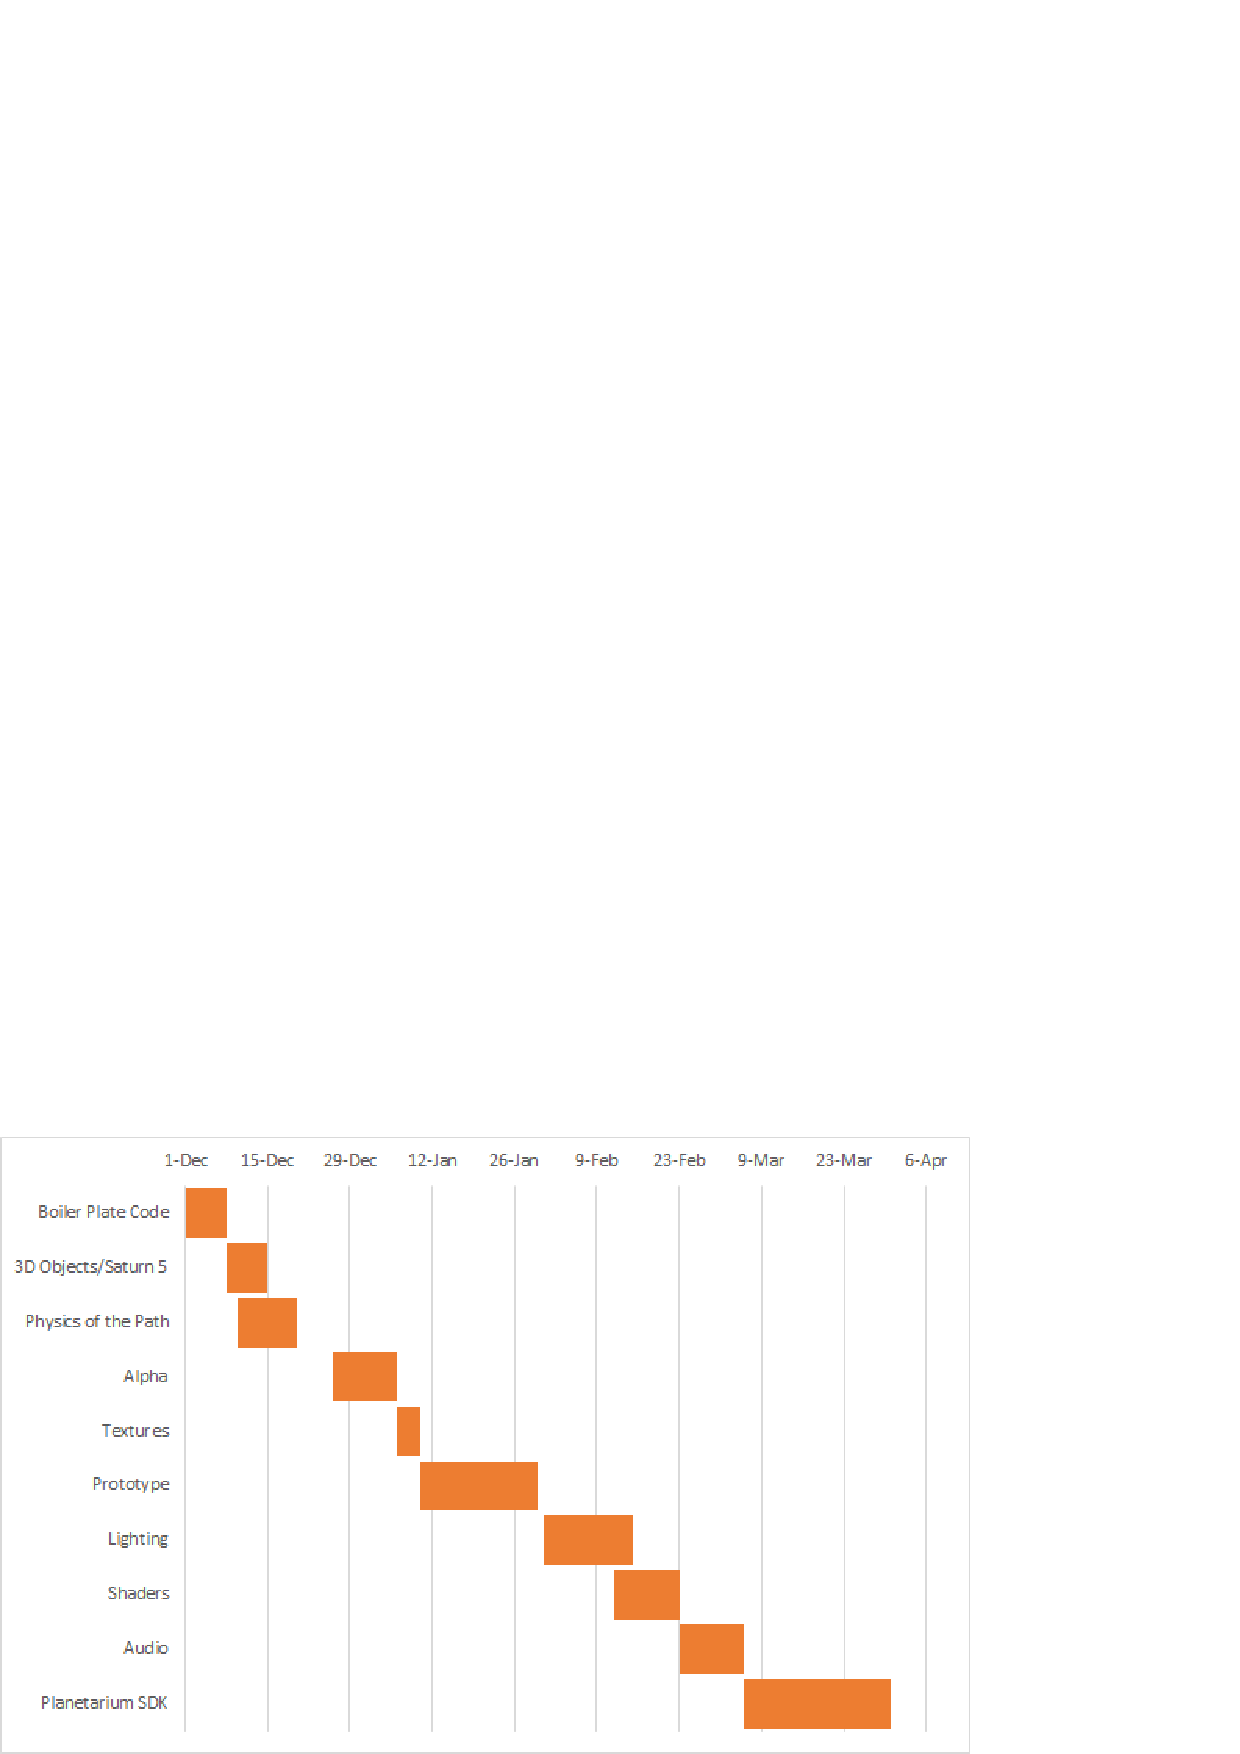
\includegraphics[width=\linewidth]{Gantt.PNG}
    \caption{Original gantt chart of proposed timeline}
    \label{fig:Gantt Chart}
\end{figure}


%%%%%%%%%%%%%%%%%%%%%%%%%%%%%%%%%%%%%%%%%%%%%%%%%%%%%%%%%%%%%%%%%%%%%%%%%
%%%%%%%%%%%%%%%%%%%%%%%%%%%%%%%%%%%%%%%%%%%%%%%%%%%%%%%%%%%%%%%%%%%%%%%%%
\section{Design Document}

\begin{titlepage}
    \begin{singlespace}


\includegraphics[height=2cm]{OSU_horizontal_2C_O_over_B.eps}   
        \par\vspace{.2in}
        \centering
        \scshape{
            \huge CS Capstone Design Document \par
            {\large\today}\par
            \vspace{.5in}
            \textbf{\Huge\CapstoneProjectName}\par
            \vfill
            {\large Prepared for}\par
            \Huge \CapstoneSponsorCompany\par
            \vspace{5pt}
            {\Large\NameSigPair{\CapstoneSponsorPersona}\par}
            {\large Prepared by }\par
            Group\CapstoneTeamNumber\par
            % 5. comment out the line below this one if you do not wish to name your team
            \CapstoneTeamName\par 
            \vspace{5pt}
            {\Large
                \NameSigPair{\GroupMemberOne}\par
                \NameSigPair{\GroupMemberTwo}\par
                \NameSigPair{\GroupMemberThree}\par
            }
            \vspace{20pt}
        }
        \begin{abstract}

        % 6. Fill in your abstract   
    
The Summer of 2019 will be the 50th anniversary of the Apollo 11 moon landing and our group, `The Apolloers', is working to create a 3D animation of the mission. This animation is being made for Jim Todd at OMSI so the animation can be displayed as part of their 50th anniversary exhibit. This document will show how we have organized the project and offer different design viewpoints so that stakeholders can see how the project has been structured. 

        \end{abstract}    
    \end{singlespace}
\end{titlepage}

\newpage
\pagenumbering{arabic}
%\tableofcontents
\subsection*{Revisions}
\begin{tabular} {|p{4cm}|p{5cm}|p{6cm}|}
\hline
Section & Original & New \\ \hline
3.5.2 - The Flight Path & \begin{itemize}
  \item We will use a data set to create the flight path
\end{itemize} & \begin{itemize}
  \item A data set would be ideal, but we will need to create our own
\end{itemize}\\ \hline
3.5.3 - Planetarium SDK & \begin{itemize}
  \item Unsure of how to show our animation in the planetarium
\end{itemize} & \begin{itemize}
  \item OMSI uses a unique scripting language for implementation in the planetarium
\end{itemize}\\ \hline
4.2 - Composition & \begin{itemize}
  \item Go through mission from launch to splashdown
\end{itemize} & \begin{itemize}
  \item Beginning and end with historic video, middle for interactive views
\end{itemize}\\ \hline
4.4 - Dependency & \begin{itemize}
  \item Mostly dependent on flight path and mission time
\end{itemize} & \begin{itemize}
  \item Dependent on the story-line that we created (Beginning, middle, end)
\end{itemize}\\ \hline
4.5 - Information & \begin{itemize}
  \item Focused on flight path information
\end{itemize} & \begin{itemize}
  \item How to make the scene realistic through size and positioning
\end{itemize}\\ \hline

\end{tabular}

% 7. uncomment this (if applicable). Consider adding a page break.
%\listoffigures
%\listoftables
\clearpage

% 8. now you write!

\subsection{Overview}
       \subsection{Scope}
        This document focuses on the 3D animation for the Apollo 11 Mission that will be created by our group, "The Apolloers" for display at OMSI. The design principals of the project will be outlined here, as well as design elements, such as functionality, usability, and requirements. These principals and elements will outline the deliverables of our project as well as the resources needed to complete it. The context, stakeholders, and intended audience our project will be used in will also be outlined, which will provide supplementary reasoning for our chosen delivarables. 
        
    \subsubsection{Purpose}
        The design and structure of this project will be outlined so that readers would be able to understand how the 3D animation is organized from a development viewpoint. In addition to the readers, this document will also serve as guidelines for our group to follow throughout the year. This document will be changed throughout the year as we refine our design. 

    \subsubsection{Intended Audience}
        This document is intended for the stakeholders of the Apollo 11 3D animation, as well as any interested group that would like to know more about how the animation is structured. Some main takeaways of this document are the design, structure, and connectivity of the components of our animation, so that readers would have a general idea of how to make a similarly structured project. 

\subsection{Definitions}

\begin{tabular} {|l|p{13.5cm}|}
\hline
Term & definition \\ \hline
API & An Application Programming Interface is a set of protocols and tools that are used to build a software application. Essentially the `building blocks' that a programmer uses to build an application.  \\ \hline
Apollo 11 Mission & A spaceflight operated by NASA to land the first humans on the Moon, launched July 16th, 1969.  \\ \hline
Graphics Pipeline & A conceptual model that describes the steps that a graphics system needs to perform in order to render a 3D scene. \\ \hline
High/Low Poly & The amount of polygons used to make a 3D model, impacting performance.\\ \hline
NASA & The National Aeronautics and Space Administration is a federal agency that focuses on research and development related to air and space.	\\ \hline
OMSI & The Oregon Museum of Science and Industry, located in Portland, Oregon	\\ \hline
OpenGL & An open-source graphics library API that is used to interact with graphics hardware to design 3D renderings.	\\ \hline
SDK & A Software Development Kit is a set of tools that program developers use to write programs for an application. \\ \hline
Polygon Count & Refers to the number of polygons in a scene. The more polygons in the scene, the more time it takes for the scene to be executed, often resulting in lag. \\ \hline
SkySkan & A company that provides planetarium software and equipment to OMSI. \\ \hline

\end{tabular}

\subsection{Design Description}

    \subsubsection{Design Stakeholders}
    The stakeholders for our project are OMSI, as well as the audiences who will be viewing our video. The educational and technical quality of our video will reflect on OMSI. The planetarium audiences will also be affected by the technical and educational quality of our video. If the video is more entertaining than educational, then the audience will not understand the impact and ambition of the Apollo 11 mission. If the video is more educational than entertaining, then the audience will be bored and less likely to pay attention to the content of the video.
    
\subsubsection{Design Views}
    The Apollo 11 animation project can be broken into different views that can all be used to describe the animation. This document will look at the design of the animation through the different viewpoints listed below, and will explain those viewpoints in detail in Section 4. 
    
    \subsubsection{Design Viewpoints}
    \begin{enumerate}
        \item \textbf{Context}: In what context will this animation be viewed.
        \item \textbf{Composition}: How the animation is separated into different entities.
        \item \textbf{Logical}: What logic is constant throughout the animation, regardless of design decisions.
        \item \textbf{Dependency}: How different entities of the animation depend on others.
        \item \textbf{Information}: What data will be needed and how it will be used in the animation. 
        \item \textbf{Interface}: How developers should correctly use the animation.
        \item \textbf{Resources}: What external entities are needed for the animation. 
    \end{enumerate}
    
    \subsubsection{Design Elements}
    There are many elements of a 3D animation that all need to work with the other elements to produce a quality project. The programming platform OpenGL will be used for managing the elements relating to 3D graphics. Since we are building for a Windows platform, we will also make use of Windows system calls as needed.
    
    The programming in OpenGL will dictate what 3D objects are in the project, where they are in the scene, and how they look. Many 3D objects in our project will come from an online repository, which we may need to add textures to, which would also be found online. Since the source for each object will likely be different, proper scaling will need to be applied to keep the size realistic. Once a 3D object is in the scene, different lighting features will be programmed in to account for the Sun and that light reflecting off of the other objects. Then to make objects move, key-frame animation will be used to interpolate the path between a start and goal point. 

    \subsubsection{Design Overlays}
	
	\subsubsection{Textures and 3D Models}
	Textures will be needed for some of our 3D objects, such as the Earth and Moon. Most of these textures will come from the NASA websites, which are readily available for public use. It is notable that these textures have been created with great detail, meaning that the textures may slow the program, or look out of place if near a lower quality texture. 
	
	The 3D model of objects such as the Lunar Module will likely be obtained from a model sharing site. We will attempt to find low-poly objects for our initial program so that the playback is not slowed down. High-poly objects may look better, but take many more resources to load. When our program is implemented at OMSI, Jim Todd should have industry quality models that can be used in the planetarium with less concern for polygon count. 
	
	\subsubsection{The Flight Path}
	Ideally we would want a dataset of the whole flight and back. Using that data set, paths can be interpolated from between the sets of points, resulting in a realistic flight path. While this would be straight-forward to implement, it is unlikely that we will have access to such a resource. Instead, we will need to calculate our own flight pat. This will still be done by using data points, but we must calculate each one, so there will be far less data points, meaning a less accurate flight path.
	
	\subsubsection{Planetarium SDK}
	One of our biggest stretch goals is to integrate our animation into the OMSI planetarium. We suspect that their planetarium use an SDK to interpolate subsections of the projection, but we currently do not have access to that SDK. Our contact here at OSU, Mike Bailey, has been in touch with SkySkan to determine how to best go about the process to implement an animation. It appears that there is a unique scripting language that is used for the planetarium. If the animation will go to the planetarium, we will use sample scripts to develop a prototype script resembling our animation for Jim Todd to test and finalize. 
    
    \subsubsection{Design Rationale}
	The basic rationale of our project is that setting the scene correctly is the most important factor in making this animation high quality. The Earth, Moon, and Sun need to be in the right position and the view port needs to be in the right position to reflect that. The lighting from the sun needs to be accurate as it reflects and refracts off the lunar capsule, Moon, and Earth. The small details matter the most, such as the Earth having its iridescent glow that is given off by its atmosphere, or both planetoids having a dark and a light side. With all of this combined, our goal is to make the audience feel as if they are watching the Apollo 11 mission live.
	
    \subsubsection{Design Languages}
	C++ is going to be our design language solely because of our choice to use OpenGL as our API. OpenGL makes use of graphics libraries that are written in C++, meaning that we must also utilize that same language. C++ gives the programmer great control over what they implement, but because of that control, this allows the programmer to make a lot of mistakes. C++ is fast and efficient like its predecessor language, C, and has more back-end libraries that can help the programmer achieve what he is trying to do. Even though these extra libraries can slow down an application, the effect is minimal for a project with a scope as large as ours. Lastly, our group will need to be cautious with memory usage because C++ does not automatically clean up memory such as some other languages, so we will need to be sure to free any memory that we allocate. 


\subsection{Design Viewpoints}

    \subsubsection{Context Viewpoint}
    
    This animation will be viewed primarily by OMSI visitors. This audience can range from young school children on field trips, to very technical industry leaders. We will want the user of this program to be able to change the viewpoint of the scene, regardless of if the user is a visitor or a staff member running the program.  
    
    \subsubsection{Composition Viewpoint}
    
    Our project will consist of a beginning, middle, and end. The beginning and end will consist of historic video related to the Apollo 11 mission to educate and provide context. The middle will allow the operator to take control of what viewpoint to see and be able to look around that view with the mouse. 3D objects, animation, audio, textures, lighting, shaders and more will all come together to create the scene. While there are not direct relationships between all these parts, they all add to the overall detail and quality of the animation. 
    
    \subsubsection{Logical Viewpoint}

    Our logic will be determined by how far into the animation the operator is. The beginning and end of the animation will be shown in a sequential fashion with little to no variation. When a certain action completes and/or a time is reached, new actions will take place. Conversely, during the middle of the animation, our program will allow changes in viewpoints. The simple logic will result from different keyboard buttons being pushed. These presses will not only change the view, but reset the previous and new scenes, this way the operator will always know what to expect when they press those keys. A stretch goal would be to allow some animations to be returned to the point in time when the last view was changed. This would be useful for a longer animation that the operator may want to pause and come back to later. 
    
    \subsubsection{Dependency Viewpoint}

    Different parts of the animation will not need to be loaded for certain viewpoints. For example, the lunar surface with an astronaut does not need to be loaded if the view is from the Earth. Each object will be given a 'flag' of sorts that we can set depending on what each view needs loaded. This will help with performance and prevent objects appearing out of place. Along these same lines, certain audio clips will be played when a view is chosen or when a certain time is reached. 
    
    Other than when to load objects, our program will not contain many actions that are dependent on others. With a graphics project such as this, all assets are loaded into memory at the beginning of running the animation so that each asset can quickly be retrieved for display to the screen. The program mainly determines when and how to display data from the computer's memory. 
    
    \subsubsection{Information Viewpoint }

    General knowledge of the Apollo 11 mission is needed to create an accurate representation in an animation. The sequence of events and a timeline are necessary, but also details such as the true size of all objects in the scene and the positioning of those objects. Because of our audience, extra care must be taken to make the animation as realistic as possible since there may be members of the audience that are quite knowledgeable about Apollo 11. When possible, all information will be acquired from an official NASA source and if that is not possible, other reliable sources will be used, such as news outlets and scientific journals. 

    \subsubsection{Interface Viewpoint}
    
   The 3D animation will be compiled into an executable file (.exe) so that the user can open the whole animation from one file. Then, the user will be able to start and stop the animation using a keyboard, and change their viewpoint by clicking and dragging their mouse, or choose set viewpoints using the keyboard. If the user does not want to change the viewpoint, the viewpoint will be set to default viewing positions that our group has chosen. The user will be able to view the video from outside of the spacecraft, inside the spacecraft, on the moon, and on Earth. 

    \subsubsection{Resources Viewpoint}
    To obtain the audio of the transmissions between the Apollo 11 crew and Tranquility Base, we will use NASA's archive of audio files from the Apollo 11 mission. Using Windows system calls, these files will be played approximately at the same stage of the mission as they were recorded in. Our group will not be implementing every audio file in the Apollo 11 audio archive, but instead we will aim to enhance the animation. The audio clips will need to be educational, but not include too much jargon for the audience. 

    Similarly to audio, our group will also need to obtain 3D models and textures from online repositories. Models will include the Command Module Columbia, and Lunar Module Eagle, an astronaut, and more. Multiple textures will be needed for the Earth and the Moon at different levels of detail, depending on how close the view port is during the animation. Finally, the background will need an accurate star-map to emphasize the vastness of space. Although, the star map needs to toggle because the stars cannot be seen from the surface of the Moon. 
    
\subsection{Conclusion}
A 3D animation consists of many different elements that all need to work together based on the implementation in a given API. We will be using OpenGL as our primary API that will manage the main graphical elements of our group's Apollo 11 3D animation. The animation will include historical context of the mission and what the mission was like on the Moon with full functioning elements such as 3D objects, texturing on those objects, lighting for the scene, etc. With a completed animation, direct users of the animation will be able to use a mouse and keyboard to navigate through the animation and view the scene through arbitrary viewpoints. Lastly, the main goal of this Apollo 11 animation is to engage audiences at OMSI and encourage curiosity in regards to the vastness of space. 

%%%%%%%%%%%%%%%%%%%%%%%%%%%%%%%%%%%%%%%%%%%%%%%%%%%%%%%%%%%%%%%%%%%%%%%%%
%%%%%%%%%%%%%%%%%%%%%%%%%%%%%%%%%%%%%%%%%%%%%%%%%%%%%%%%%%%%%%%%%%%%%%%%%
\section{Tech review}

\begin{titlepage}
    \pagenumbering{gobble}
    \begin{singlespace}
        \hfill 
        % 4. If you have a logo, use this includegraphics command to put it on the coversheet.
        
\includegraphics[height=4cm]{OSU_horizontal_2C_O_over_B.eps}   
        \par\vspace{.2in}
        \centering
        \scshape{
            \huge CS Capstone Technology Review \par
            {\large\today}\par
            \vspace{.5in}
            \textbf{\Huge\CapstoneProjectName}\par
            \vfill
            {\large Prepared for}\par
            \Huge \CapstoneSponsorCompany\par
            \vspace{5pt}
            {\Large\NameSigPair{\CapstoneSponsorPersona}\par}
            {\Large\NameSigPair{\CapstoneSponsorPersonb}\par}
            {\large Prepared by }\par
            Group\CapstoneTeamNumber\par
            % 5. comment out the line below this one if you do not wish to name your team
            %\CapstoneTeamName\par 
            \vspace{5pt}
            {\Large
                \NameSigPair{\GroupMemberOne}\par
                %\NameSigPair{\GroupMemberTwo}\par
                %\NameSigPair{\GroupMemberThree}\par
            }
            \vspace{20pt}
        }
        \begin{abstract}
        % 6. Fill in your abstract    
        	This document aims to compare OpenGL, Unity, and DirectX to see what programming platform our group will want to utilize when creating our 3D animation of the Apollo 11 mission. After the comparison, we have determined that we will be using OpenGL because it offers more control over low level graphics and because our group has already had experience developing with OpenGL. We may also utilize Unity to create a final deliverable because of better options for after effects and bundling the project together. 
        \end{abstract}     
    \end{singlespace}
\end{titlepage}
\newpage
\pagenumbering{arabic}
%\tableofcontents
% 7. uncomment this (if applicable). Consider adding a page break.
%\listoffigures
%\listoftables
%\clearpage

% 8. now you write!
\subsection{Introduction}
Our goal is to create a 3D animation of the Apollo 11 Moon Landing, including all parts between the launch and the final splashdown. This animation will be displayed in the Oregon Museum of Science and Industry (OMSI) for guests to view in the planetarium. There are many different pieces to this process such as creating the 3D objects, using physics to simulate motion, lighting of the objects, how to handle audio, and much more. My role is to compare what programming platform we will be using for most of the project. In this document, the OpenGL, Unity, and DirectX development platforms will reviewed and compared to choose what will be best for our project. The review will be based on some brief history of each system, how each platform would be able to support our needs, how easy it would be for our group to learn, and how accessible the final project would be.

\subsection{OpenGL --- ``The Industry's Foundation for High Performance Graphics''}
OpenGL is a graphics library (hence the GL) introduced in 1992 and soon became the industry standard for 2D and 3D graphics applications [1]. OpenGL is currently operated by The Khronos Group, a non-profit consortium that works with similar open standard systems [2].  Open standards mean that the standard of the product is available to the public and is often favored in software development because of the extra control developers can have, especially when it comes to development on multiple different systems (Windows, Linux, mobile, etc.). This also means that there are many Application Program Interfaces (API's) that have spawned from OpenGL, such as WebGL, a variant that allows for graphics rendering within web browsers [3].
\newline
\newline
Since OpenGL is a collection of graphics libraries, using this in our project would essentially be a C++ program that utilizes these libraries, and other libraries as needed. Working with the libraries at this level gives access to make changes at a low level (close to the hardware). This is a great advantage for custom options, but it also means that there are few “shortcuts” that can be made, so programming can be quite tedious. However, for our group specifically, we are all currently taking CS 450: Intro to Computer Graphics, taught by Mike Bailey, our OSU lead for the project. In this class, we are learning how to utilize OpenGL which means that we all have similar experience with this platform and would not require learning many more concepts. 

\subsection{Unity –-- ``The World's Leading Real-Time Engine''}
Unity Technologies ApS (formally Over the Edge I/S) was founded in 2004 and is most well-known for their development of the Unity Real-Time Engine [4]. This engine is focused on creating 2D and 3D graphics that are then placed into an environment that developers can further manipulate, giving the term ``real-time'' engine. Unity provides a graphical user interface (GUI) for developing projects so that instead of just writing code, developers have graphical menus they can use to make changes. These interfaces are also useful for artists to customize visuals, and writers to change the general ``flow'' of the project. Unity is most known for being the engine that runs ``Half of the world's games'' and for good reason since Unity is available for every major system available today [5].
\newline
\newline
Unity is an ``engine'', meaning that a lot of overhead is handled for the developer behind the scenes. This can be great for developers that do not want or need to access to low level changes and it also helps to prevent overwhelming new users when they are learning how to utilize the system. This combines with the GUI to provide a streamlined interface that is still incredibly powerful. For groups, Unity also offer built in version control systems and cloud storage [5]. This allows projects to be stored and edited in the cloud, and all those changes are documented across the group. This service is free for groups of 4 or less, but bigger groups will have to pay monthly fees. While the Unity engine is free for people to use, because Unity is run by a for-profit company, other useful programs within the engine need to be purchased through a monthly subscription [6]. 

\subsection{DirectX –-- ``Are you excited? You will be''}
The first version of DirectX was released in 1995 and has had many different versions, up to DirectX 12 that was released in 2015 [7]. DirectX is a collection of API's that is included with Microsoft Windows to handle all multimedia tasks, especially 2D and 3D graphics. Notable API's include Direct3D, DirectSound, DirectInput, DirectDraw, and many more. DirectX has been the main graphical driver for Microsoft Window's operating systems and Microsoft Xbox systems with little to no compatibility with other systems. Even though DirectX is still staying strong with Microsoft, it appears that support for DirectX 12 has been dropping for other, multi-system options such as the Vulkan API, especially when it comes to the video game industry [8].
\newline
\newline
The DirectX software development kit (SDK) is made of runtime libraries that are a layer of abstraction up from direct graphical implementations [9]. While developers will still need to understand the basics of computer graphics, DirectX will handle some of the details automatically. This being said, due to competition from other low-level API's, DirectX 12 introduced low-level programming to the system so that developers could make low-level changes to reduce driver overhead [10]. Another area that DirectX has received pressure is the fact that it only runs on Microsoft Systems. Even though it does this very well, current trends in computing favor applications that can be run on many different types of systems. 

\subsection{Comparison}
We will start by comparing OpenGL and DirectX as these are the most similar. OpenGL provides more low-level options for optimizing graphics so that they can look the best while using as few resources as possible. While DirectX 12 has introduced similar low-level programming, there are still many factors that are handled by the DirectX API itself, which can help introductory developers, but may gloss over some details. Both systems would look similar in the eyes of a developer as they would be programming in a C-style environment to take advantage of graphics libraries/API's. However, one of the most notable differences is that OpenGL is open-source (and therefore works on many different systems) while DirectX is limited to Microsoft supported systems. In today's world, with so many different sysems such as macOS, Linux, Android, IOS, etc., multi-system support is a crucial feature to have when developing multimedia graphics. 
\newline
\newline
Comparing Unity and OpenGL is more difficult because OpenGL is a collection of graphical libraries, while Unity is a graphical engine, that manages many API's, that are based on libraries. This means that OpenGL will offer much more low-level customization while Unity offers a much more user-friendly environment to bypass the low-level options that may not be important to a larger program. Unity offers an easy to use GUI so that even introductory developers can get a foothold in their project without being overwhelmed with low-level code, while OpenGL requires the developer to write code for every aspect of their graphics project. With this being said, Unity still offers low level options to customize, but often the system will take care of that for the developer. Unity also makes importing other resources much easier because of the graphical interface. OpenGL requires separate libraries and functions to include resources such as sound, but again, offers complete control over these resources. Another factor with our project is the fact that all members of our group have had recent experience with OpenGL and can use Professor Mike Bailey as a resource for OpenGL support, while we have very little to no experience in Unity and would have to learn to use the entire engine. 

\subsection{Conclusion}
All the above options, OpenGL, Unity, and DirectX, would be suitable for our 3D animation of the Apollo 11 Moon landing. However, with our limited information about how OMSI will want to implement this animation, our group will not be using DirectX because it is not supported on a wide variety of systems. Between OpenGL and Unity, our group will primarily be using OpenGL based on our experience with the system. Also, implementing the physics for the different 3D objects will be best done on the low-level system. However, once the 3D animation is complete, our Group may still utilize Unity for after effects, adding audio to the presentation, and making a deliverable that is easy to use. It is too early to guarantee this, but the tools that Unity offers could make combining all our resources together much smoother than trying to program every aspect in OpenGL. In the end, our main goal is to produce a deliverable to be shown at OMSI and then shared with others, so as the project progresses, our group will use whichever systems we can to best achieve this goal. 


\subsection{References}
\begin{enumerate}
\item [1] Group, K. (2018). OpenGL - The Industry Standard for High Performance Graphics. [online] Opengl.org. Available at: \url{https://www.opengl.org/} [Accessed 31 Oct. 2018].
\item [2] The Khronos Group. (2018). The Khronos Group. [online] Available at:\url{https://www.khronos.org/} [Accessed 31 Oct. 2018].
\item [3] MDN Web Docs. (2018). WebGL: 2D and 3D graphics for the web. [online] Available at:\url{https://developer.mozilla.org/en-US/docs/Web/API/WebGL_API} [Accessed 31 Oct. 2018].
\item [4] Bloomberg.com. (2018). Company Overview of Unity Technologies, Inc.. [online] Available at:\url{https://www.bloomberg.com/research/stocks/private/snapshot.asp?privcapId=241908542} [Accessed 31 Oct. 2018].
\item [5] Unity. (2018). Unity. [online] Available at: \url{https://unity3d.com/} [Accessed 31 Oct. 2018].
\item [6]Unity Store. (2018). Store - Unity Store. [online] Available at: \url{https://store.unity.com/} [Accessed 31 Oct. 2018].

\item [7]	Codingunit.com. (2018). The History of DirectX | CodingUnit Programming Tutorials. [online] Available at: \url{https://www.codingunit.com/the-history-of-directx} [Accessed 1 Nov. 2018].
\item [8]	Smith, R. (2018). Comparing Vulkan \& DX12 API Overhead on 3DMark. [online] Anandtech.com. Available at: \url{https://www.anandtech.com/show/11223/quick-look-vulkan-3dmark-api-overhead} [Accessed 1 Nov. 2018].
\item [9]	M. Satran, “Getting Started with DirectX Graphics,” Microsoft Docs. [Online]. Available at:\url{https://docs.microsoft.com/en-us/windows/desktop/directx} [Accessed 01 Nov. 2018].
\item [10]	Channel 9. (2018). Direct3D 12 API Preview. [online] Available at:
\url{https://channel9.msdn.com/Events/Build/2014/3-564} [Accessed 1 Nov. 2018].

\clearpage
\end{enumerate}

%%%%%%%%%%%%%%%%%%%%%%%%%%%%%%%%%%%%%%%%%%%%%%%%%%%%%%%%%%%%%%%%%%%%%%%%%
%%%%%%%%%%%%%%%%%%%%%%%%%%%%%%%%%%%%%%%%%%%%%%%%%%%%%%%%%%%%%%%%%%%%%%%%%
\section{Blog Posts}
\subsection* {Dean Akin's Blog Posts}
\begin{longtable} {|p{1.5cm}|p{13.5cm}|} \hline
Fall: Week 4 &
As of right now we have finished our full problem statement, the main issue that we had to overcome is to make a good performance metrics section that portrayed it well, before we didn’t know how to write it. Due to time constraints and family issues on my part I was unable to meet with them Friday but nonetheless we finished it over google docs/github. We plan on meeting with Mike to go over requirements for our project next week. \\ \hline

Fall: Week 5 &
All we have to do is do our requirements document, everything is going pretty slow as of right now. Next week it will pick up. \\ \hline

Fall: Week 6 &
Tech reviews took awhile but all of them got done, still a slow week but documentation is always very small. Everything was smooth sailing for this week, we are planning on working together next week heavily on the design document, as planning correctly this term will decide how it will go next week.  \\ \hline

Fall: Week 7 &
The tech review didn’t take much, we are just waiting for the design document. \\ \hline

Fall: Week 8 &
We are currently hashing out the Design document this weekend, everything else seems to be okay. I am doing some pre-development for my final project for CS450 with Mike Bailey, as a proof of concept, and setting the scene. \\ \hline

Fall: Week 9 &
The only thing happening this week is working on the Requirements document over the weekend via pushing and pulling from github. Nothing else is happening due to a short week because of thanksgiving.  \\ \hline

Winter: Week 1 &
For progress we met up with Jim Todd at OMSI, he showed the WHOLE planetarium system and its API. We have a more solid understanding on what we want to do, and piping our animation into their system might of been easier than what we thought. We also met with some of the members of their research teams and asked for their opinion on what we should do and received feedback from them, and we headed home. No problems arised since then. We plan on starting development on storyboarding next week, other than that we are doing our required meetings.  \\ \hline

Winter: Week 2 &
We have managed to plan out certain things that we want to do at certain points of the animation. We have considered using key-frame animation as to have smooth interpolation of the ship and many other moving parts of the animation. Other than that we have been working on our elevator pitch and poster draft, not much has been going on. We plan to set the scene for the moon and to set up the work environment for our animation for further progress in the future early next week. \\ \hline

Winter: Week 3 &
We have drawn up a skeletal structure of our storyboard, and have decided which points in the animation can be interacted with and which are not. We have a clear goal on what we want to do to tell the best story that we can about the Apollo 11 mission, and next week we are planning to go into more detail on what we want to do within sub-scenes within the animation, and how we may do that. We are going to comprise what we wrote down into a document for Mike Bailey so that we can receive feedback on what we can further do to achieve what we want to do. \\ \hline

Winter: Week 4 &
Shannon is figuring stuff out on the audio/video stuff and the Lunar Module descent look at function. I am focusing on the key frame animation of Neil and lighting, and Jon is focusing on position of everything. As of right now, we are planning to delve more into the sound boarding than we did before. \\ \hline

Winter: Week 5 &
This week I worked on creating a key frame class while consulting Mike on what to do, during the meeting with Mike we also learned about the syntactic language that the proprietary software of the planetarium, and that Mike needs to write a MTL parser so we can read the material parameters for the objects which we loaded in. Other than that, we are tweaking position, rotations, etc, and plan on doing the same next week progressively. \\ \hline

Winter: Week 6 &
I continued on working ont he keyframe class, but ran into some issues. I cannot get it to reset so I am going to be working on that all week. \\ \hline

Winter: Week 7 &
We are finally able to get some headway on the project, I have finished per fragment writing and have been working heavily on the project while Shannon and Jon have been working on the progress report. Next week I will be working hard on the keyframe class implementation which is a big part of our project. Otherwise we keep going. \\ \hline

Winter: Week 8 &
Per fragment lighting is done, and I am almost done with the .mtl file parser to get the material parameters for the objects in the scene. Jon has gotten pretty much all of the big positioning done and Shannon has gotten something to work with the video. Next week I will be completing keyframing and animation so that things are moving. \\ \hline

Winter: Week 9 &
I am finally onto the lighting with the Earth, and how to combine all three textures into one. I have a general jist of what I want to do, but I have to write out what I specifically want to do.  \\ \hline

Winter: Week 10 &
I have finished some animation, as well as high res, blended texture of the Earth, to simulate the horizon in the original Earthrise picture during the Apollo 11 mission. For next week, I will be loading in the new lunar module/craft obj that we have received and will be adding some of our more common animations. Its basically cleaning up for the beta. No problems have arisen as of yet. \\ \hline

Spring: Week 1 &
I’m just finishing up Keyframing as it crashed magnificently, and then handing it off so Jon can do the flight path.  \\ \hline

Spring: Week 2 &
I finished keyframing and am working on an animation using it before the code freeze, otherwise all requirements are done and we just need to add more content. \\ \hline

Spring: Week 3 &
All I am doing this week is producing the wireframes of the animations I would like to do.  In the next following weeks I will do implement them and tweak them.  \\ \hline

Spring: Week 4 &
A test animation has been put up, but I am not sure why it very rigid in movement. Further investigation is needed, it is more than likely a simple error as it always is but we will see. Looking around in the animation moves smoothly. \\ \hline

Spring: Week 5 &
I added some in person perspective animations, and I am testing out why it seems so choppy. As of right now I am just adding more and more, soon I’ll get onto adding the textures onto the models. But that’ll be next week. \\ \hline

Spring: Week 6 &
I finally was able to move the eye position, and it was literally because of a type casting issue. Otherwise I’m adding all the animation as well as fine tuning performance on the animation.  \\ \hline

\end{longtable}


\subsection* {Jonathan Ropp's Blog Posts}
\begin{longtable} {|p{1.5cm}|p{13.5cm}|} \hline
Fall: Week 4 & 
We met with our TA, Richard Cunard, and got to bounce some ideas off of each other about how we are going to implement our 3D animation. Right after that meeting, we then met with our Client, Mike Bailey. We were able to get a few more details about the project and start thinking about what all we are going to need to start implementation. We started a shared document that is a list of things that we will need to know, and during our next meeting, we are going to discuss them and start breaking the list up into groups for us to work on. Lastly, we were able to finish our group problem statement and submit that assignment. Our biggest problem with that was that because our project is (objectively) straightforward, we put our document together and was still a bit short of the word count target. But, we were able to elaborate on a few portions and we look forward to getting the requirements document started. \\ \hline

Fall: Week 5 & 
This week we were unable to meet with our client, Mike Bailey, because they were out of town. We did still get to meet with our TA, Richard Cunard, and we were able to get some pointers for the requirements draft and the tech review draft. As a group, we met twice to work on the requirements draft, and finished it. Since the deadline was extended, we have not submitted so that we can have more time to read over it to check for errors and make additions.

We were seeming to have a bit of a hard time coming up with enough topics for the upcoming tech review draft. We were able to figure out the three sections that each of us will work on: How we are going to get/use 3D models, audio, and then what coding languages/interfaces we will use. Hopefully we will be able to look at these more and flesh them out before our next meeting so that we can discuss if we have any issues.

We plan to continue working on documents as assigned and meeting with our client/TA. Hopefully we will be able to review the requirements document with Mike next week to get his input. \\ \hline

Fall: Week 6 & 
This week we were able to meet with our client, Mike Bailey, and review our Requirements Draft. We received great feedback as well as having the opportunity to delve a bit deeper into some of the details of our project. We talked about everything from how audio of the mission was broadcast open mic, to the orbital mechanics that we will need to implement in our animation. Also, we discussed topics that each of our group members could write about for our tech review document; we decided to focus on the programming platform we will be using, and how to best integrate 3D objects and mission audio into the project.

Our group has still not had direct contact with our OMSI client, Jim Todd, and we brought that up with Mike. Mike offered to reach out to Jim and ask how involved with the process he would like to be, ranging from not at all, to sending technical documents and scheduling a trip to OMSI soon. Hopefully we will have a better idea about communication will look between our group and OMSI next week. \\ \hline

Fall: Week 7 & 
It has been a quiet week as our group has been working on finalizing our individual tech review documents. We were able to meet with our TA, Richard Cunard, and received more feedback on our requirements document, tips for the tech review, and a quick description of what our design document will be. After this, we were unable to meet with our client, Mike Bailey due to scheduling conflicts. We hope that early next week we can start getting an outline put together for our upcoming design document, getting advice from Richard and Mike. \\ \hline

Fall: Week 8 & 
As always, we met with our TA, Richard Cunard, and our client, Mike Bailey. With Richard, we discussed the layout for the design document that is coming up. We also learned about the 30 minute progress video that we will be needing to make by the end of the term. Then with Mike, we talked about what we learned in our tech reviews and that sparked conversations of development that will be great for our upcoming document. We have also heard back from our OMSI client, Jim Todd, through Mike, and Jim was happy with our design document. We hope to send Jim our design document and then after, all other documents for verification. Then lastly, our group is going to meet over the weekend to work on, and hopefully, finish the design document, as well as starting to set up our progress video. \\ \hline

Fall: Week 9 & 
With this being the week of Thanksgiving there is not too much to update. We were able to meet with our TA, Richard Cunard, and got a lot of clarification about our upcoming Design Doc. We also discussed the upcoming Client Verification and decided that we need to check in with Kevin and/or Kirsten to see if getting verification from Mike Bailey will be enough, or if we should try to get Jim Todd to sign off as well. Unfortunately, Mike had to cancel our weekly meeting, but we should be good to meet next week to cover the last two weeks of the term and what we should work on during Winter break. Our group has met to work on the Design Document and we have a decent outline, but we have a lot of details to add before we turn it in. Once that is done, we will start getting a plan for our progress video document and slides. \\ \hline

Winter: Week 1 &
During Winter break, our group, including Mike Bailey, drove to OMSI and met with our OMSI contacts, mainly Jim Todd. Jim was able to show us all the inner workings of the planetarium (Which was awesome!) and we got much more information about this project. This meeting was very good because I think that we all had something else in mind than what Jim had been thinking. This will mean that we need to go through all our documentation and change a decent amount, but all should be good.

We have scheduled weekly meetings with Mike for Fridays at 4 PM, and today we talked about our overall storyboard for the animation and some of the new goals that we should aim for. I think it really energized our whole team and we will start getting a basic scene put together for next week. Mike also let us know that he will be in touch with Sky-Skan (Planetarium software company) for more details of how we can possibly integrate an OpenGL project. Regardless of what will actually work with the planetarium, we will be making an OpenGL animation, at least to figure out positioning for our objects. \\ \hline

Winter: Week 2 & 
We met with Mike this week and we are still waiting on Sky Skan, but have only recently reached out. In the meantime, we are working on getting a general storyboard together for the animation. This will let us know what objects we need to load into the scene, where to place them and when. Also, a general story of the animation will be made so that we know what parts to focus on during viewing. 
\\ \hline

Winter: Week 3 &
This week we worked on finalizing our storyboard for our animation. We will run it by Mike for a final analysis during next week's meeting, but we have a solid idea of what story the animation will tell. During our meeting with Mike this week we talked about how to load in certain objects into OpenGL (Use blender to make things .obj). A small problem that came up is that Mike has still not heard back from SkySkan (planetarium software company) but that is not too critical. 

Our next goal is to get the lunar surface ready so that we can load in other objects and set the scene. We also discussed how to keep Jim Todd at OMSI updated and we will probably have one web meeting during the term about storyboarding and then make a trip to OMSI near the end of the term to test an alpha of the animation. 
 \\ \hline

Winter: Week 4 &This last week we worked to load in the lunar landing site and set up more of the scene. We also finalized our storyboard, though, after our meeting with Mike, we will likely re-format the storyboard to be more useful when setting up the OpenGL program. Also during our meeting with Mike, we found out that SkySkan has gotten back to Mike and they are excited to help out. It sounds like to display in the OMSI planetarium, we will need to use the software's unique scripting language, but after seeing some samples, it seems doable. We will still use OpenGL to plan out viewpoints and show a demo at Expo. 

Our main goal is to get an Alpha up and running for class. Some basics we want to include for this are all main objects loaded in the scene, some main viewpoints set up, and a general animation that navigates through the scene (Mainly the lunar surface and earth to moon). If possible, we would also like to load in a video and audio clip. 
\\ \hline

Winter: Week 5 & This week did not have any major updates as we are still working on getting an alpha ready. We did finally get to get a poster critique meeting and we got great feedback from Kirsten and group 72, we will focus more on what we created instead of the Apollo 11 mission. We also met with Mike again and he has gotten more info from SkySkan about scripting for the planetarium. For now, he is gathering all that and we are going to just focus on the OpenGL program for this term, switching to the scripting next term. 

This coming week is crunch time for the alpha. We need to finalize all positions, get lighting, get textures, get a demo animation path, and figure out how to load videos to OpenGL. We had assigned these parts to each of us and hope to get everything going this week. 
\\ \hline

Winter: Week 6 & 
Not much to tell this week other than continuing work on the Alpha. Work is going well with only problems coming up with incorporating video with OpenGL, but we are hoping to get help from Mike to make this a possibility. Overall, we should hit our goals for Alpha if work continues as planed. 
\\ \hline

Winter: Week 7 & 
Last week we were able to finish our Alpha with most of the features that we were aiming for (got stuck on playing videos and finding a flag object), but we are happy with it, as well as Mike. This week we all took some time for other classes but still are going to have our progress report finished by Monday. 

After our TA meeting, we did get more information about how we need to communicate our goals for the project. The OpenGL animation is a must-have for Expo, meaning that the script for the planetarium, while it is our main deliverable to OMSI, is going to almost be labeled as a stretch goal in terms of Expo and such. 

Meeting with Mike this week, we decided that we will try to make it to OMSI at the end of finals week and try to have some sort of simple script to try out to see if we are on the right page. We then reviewed what we need to get done for our beta and got a plan together for the rest of the term. 
\\ \hline

Winter: Week 8 & 
This week I worked on fine-tuning the positioning in the scene. Now the exact location of Tranquility base is marked and the Lunar Module is in the correct place on the lunar surface. Also, the Earth has been rotated to the correct angle as if you were on the Moon. Dean and Shannon have also worked on textures, key-frames, and audio.

My next goal is to figure out how to play video, which will probably give rise to some issues, but hopefully, I can get something working this week. Otherwise, we are still just working towards Beta. 
\\ \hline

Winter: Week 9 & 
This week our main struggle was with implementing video in OpenGL. We tried a few AVI libraries, ffmpeg, and OpenCV, and we ran into issues with all of them. After talking with Mike Bailey, we decided that play video at Expo was not a priority and that we should use that time to improve other parts of the project. 

In our meeting with Mike, we went over what we want to have done for our trip to OMSI at the end of the term (essentially for Beta). We need animated views and a cloud texture on the Earth. We also talked about other fine-tuning things (rounding the lunar surface, re-arranging things for viewpoints, LM texture). 

For the Lunar Module texture, we found out that all we have is color. This is a free object from NASA's Github, so we are considering purchasing one of better quality. Whatever we decide, the Lunar Module probably will not be textured for Beta, and we are fine with that. And lastly, we talked about documentation, updates to our poster, and questions to ask Jim at OMSI. 
\\ \hline

Winter: Week 10 & 
\\ \hline

Spring: Week 1 & While not much progress was made during spring break or this first week back, the Friday before break our team did drive to OMSI to meet with our client, Jim Todd again. Jim was happy with the progress we have been making and we put together a better plan for implementing our animation at OMSI's planetarium. But for now, we still need to focus on being ready for Expo.

Today we had our weekly meeting with Mike Bailey and went over what we need to do for this term. First, we want to essentially be ready for Expo by the code freeze. This would mean finalizing textures, more animations, and general fine-tuning. During this time, we would also make final changes to our documentation/poster. Then, we would shift our focus to creating the final project for use at OMSI. This will mostly take form of a unique script to be used by their Dark-Matter software. 
\\ \hline

Spring: Week 2 & This week we were unable to meet with Mike Bailey, but we plan to send our updated documentation to him for review. After we make any changes, we will send it to Jim Todd at OMSI. Also, since we could not meet with Mike this week so we do not have a system ready to read the texture associated with the new Lunar Module model that we got. So unfortunately it will not be ready for the code freeze, but all other aspect should be ready by Monday. 

Dean finished some animation code that we will get to work with this weekend and we are hoping to retrieve some more sources for audio and video clips. Lastly, the flight path needs to be finished and hopefully animated by Monday.
\\ \hline

Spring: Week 3 & 
This week was fairly quiet after getting the code freeze turned in. We made finishing touches to our documentation and sent it to Mike and Jim for verification. Unfortunately we have not gotten a response from Jim yet, but we will send a verified copy to Kirsten as soon as we do. We did still meet with Mike and we got feedback on our poster, then we went over a few more things that we need to do before Expo and then we divided up the work. We have some more animations to make and general fine-tuning of the project, but the next few weeks should be relatively slow before Expo. 
\\ \hline

Spring: Week 4 & 
This week we all continued work on additional animations and all individually ran into some delays. I have not found the best way to organize the animation for the flight path. Shannon is having issues with alpha masking the landing site. Dean's keyframes are not as smooth as they should be. Hopefully, these can be worked out in the coming week. 

We also made finishing touches to our poster and turned it in, but Mike still has not gotten the lunar module textures working, so we hope to have that finished after this weekend so we can add a textured screenshot to the poster before printing. 
\\ \hline

Spring: Week 5 & 
This week each of us made progress towards our individual animations. We also finished and submitted the final version of our poster for printing. We are feeling good with the expo and are hoping to have the project essentially done next week, that way we have a week to prepare for expo directly. 
\\ \hline

Spring: Week 6 & This week we all continued to prepare for the engineering expo next week. We worked with engineering IT to get a desktop computer to use with a 1080 ti graphics card. Our animation has been tested on this and is currently in Mike Bailey's office. This weekend, we plan to meet and produce the final animation for expo, along with any final preparations. 
\\ \hline

\end{longtable}


\subsection* {Shannon Sandy's Blog Posts}
\begin{longtable} {|p{1.5cm}|p{13.5cm}|} \hline
Fall: Week 1 & \\ \hline
Winter: Week 1 & \\ \hline
Spring: Week 1 & \\ \hline
\end{longtable}

%%%%%%%%%%%%%%%%%%%%%%%%%%%%%%%%%%%%%%%%%%%%%%%%%%%%%%%%%%%%%%%%%%%%%%%%%
%%%%%%%%%%%%%%%%%%%%%%%%%%%%%%%%%%%%%%%%%%%%%%%%%%%%%%%%%%%%%%%%%%%%%%%%%
\section{Poster}
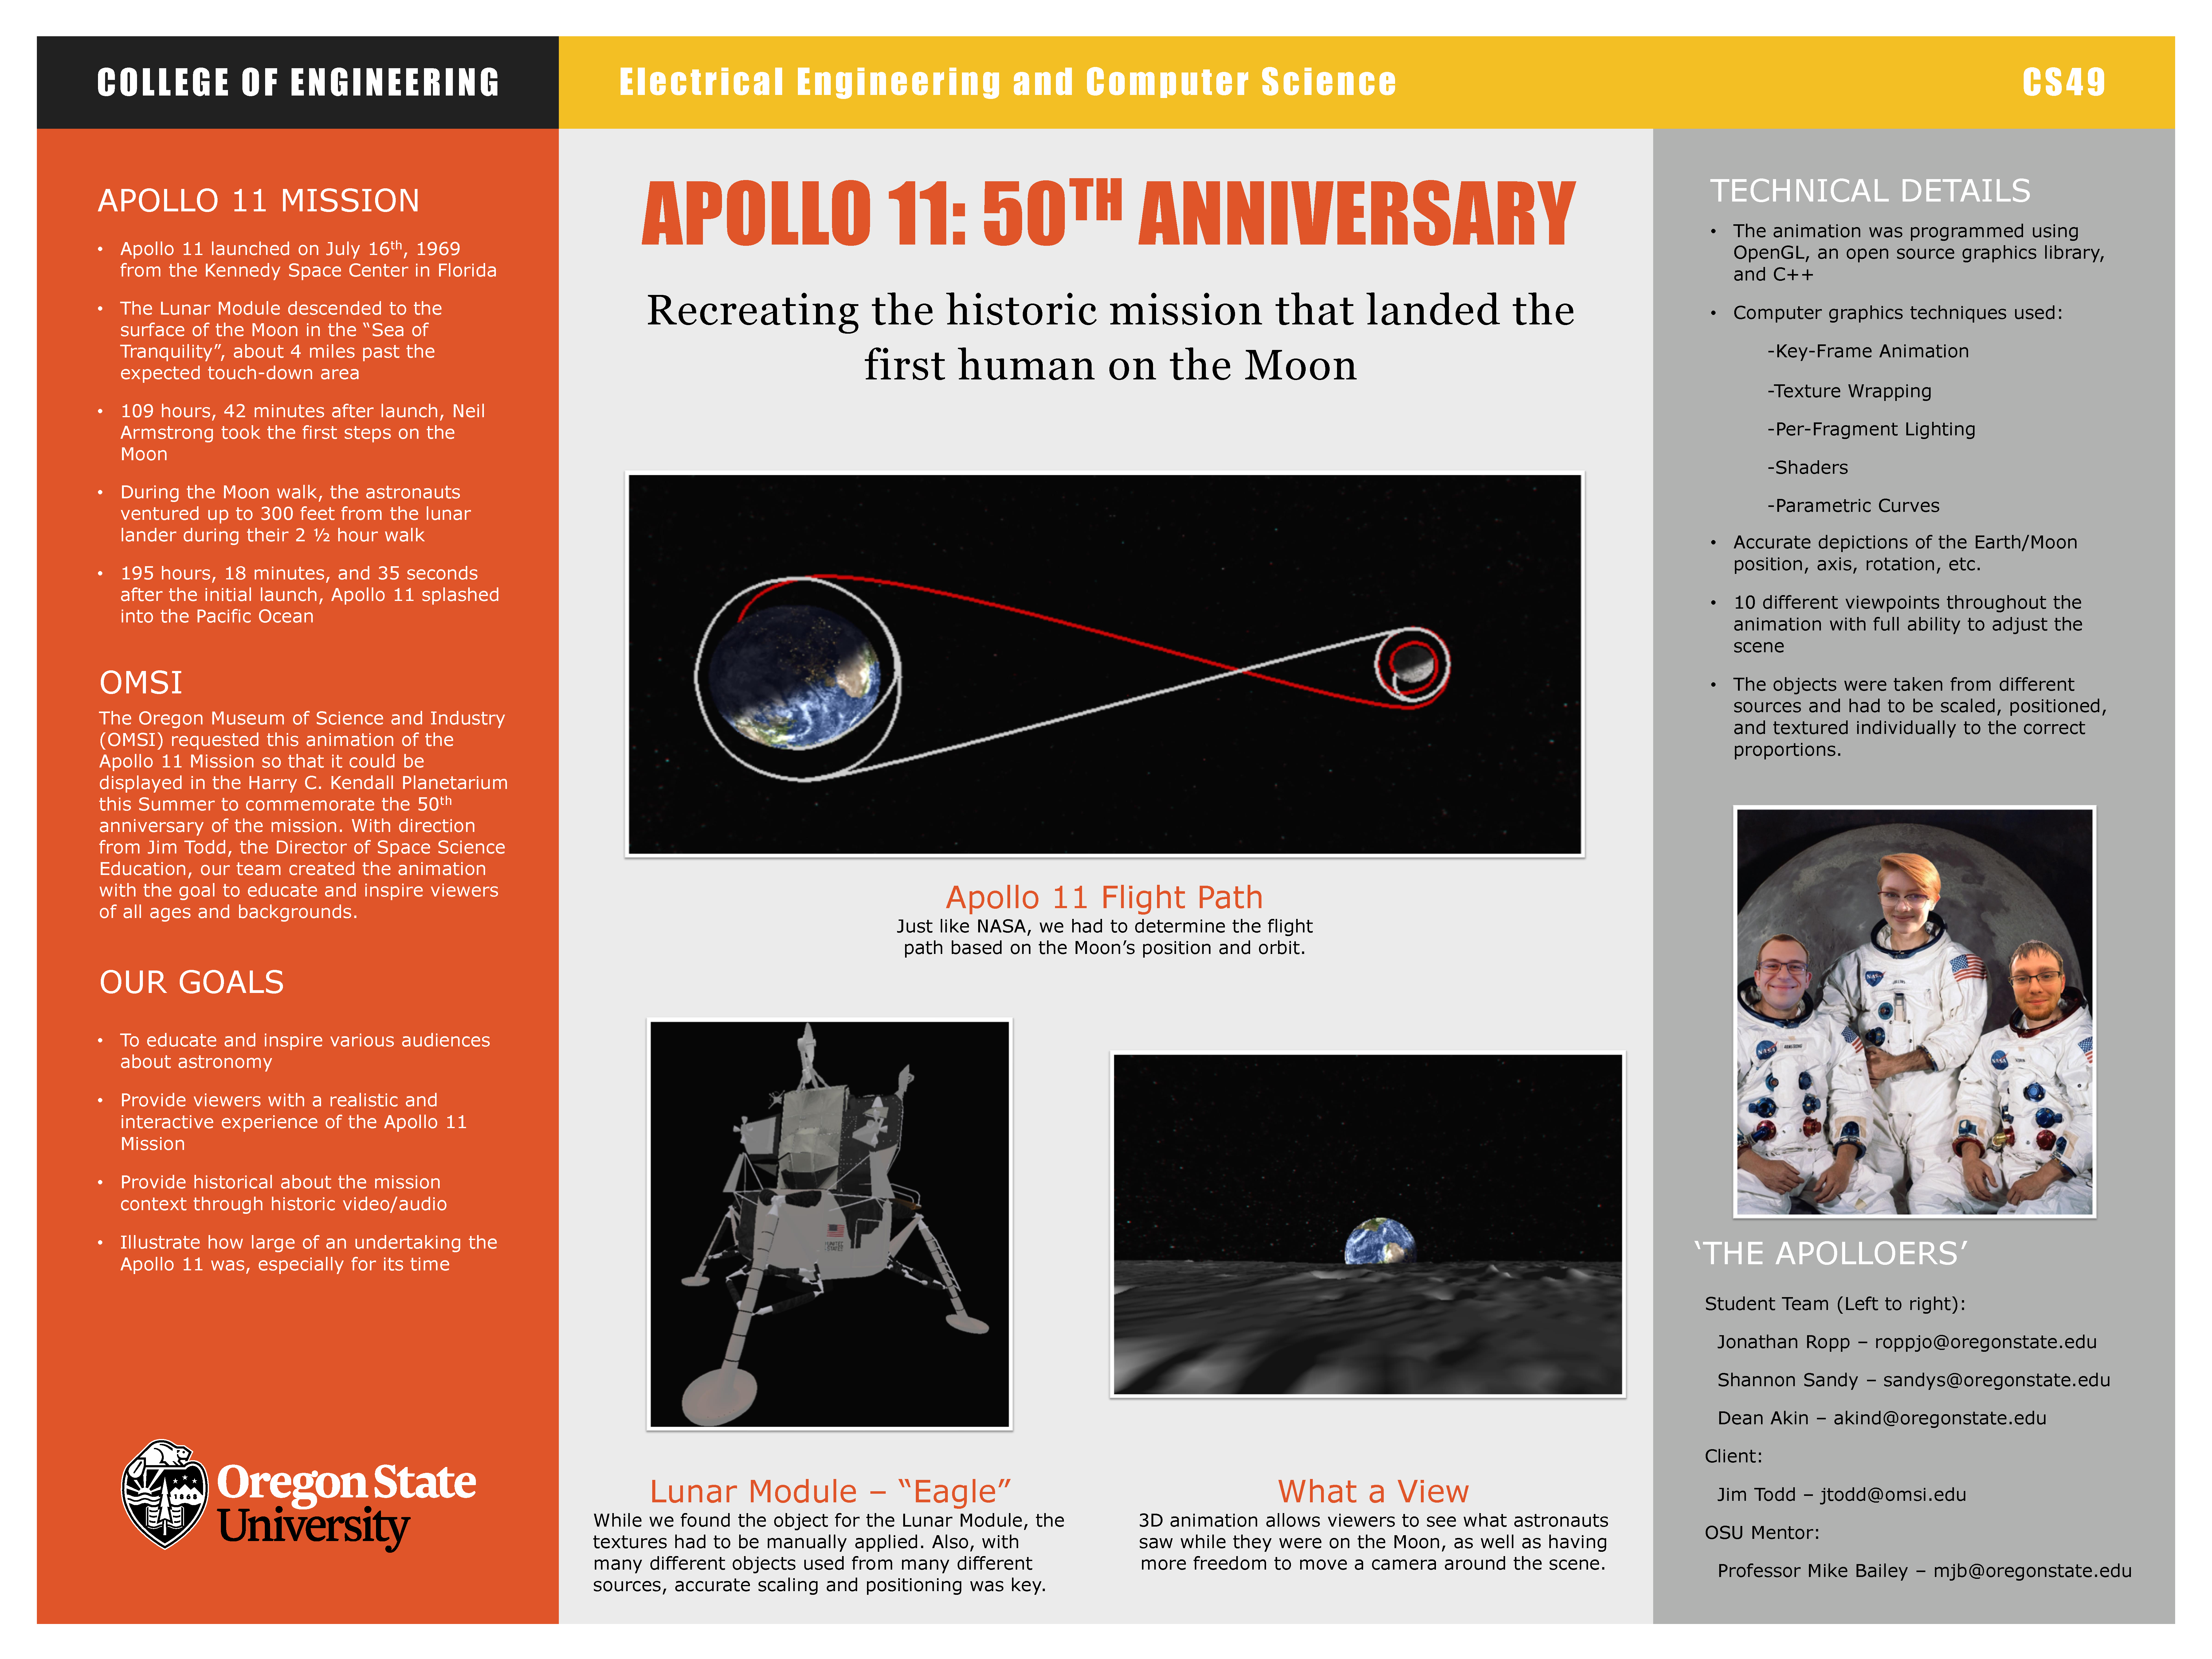
\includepdf{Group49_Poster.pdf}

%%%%%%%%%%%%%%%%%%%%%%%%%%%%%%%%%%%%%%%%%%%%%%%%%%%%%%%%%%%%%%%%%%%%%%%%%
%%%%%%%%%%%%%%%%%%%%%%%%%%%%%%%%%%%%%%%%%%%%%%%%%%%%%%%%%%%%%%%%%%%%%%%%%
\section{Project documentation}



%%%%%%%%%%%%%%%%%%%%%%%%%%%%%%%%%%%%%%%%%%%%%%%%%%%%%%%%%%%%%%%%%%%%%%%%%
%%%%%%%%%%%%%%%%%%%%%%%%%%%%%%%%%%%%%%%%%%%%%%%%%%%%%%%%%%%%%%%%%%%%%%%%%
\section{Resources}

Our most valuable resource was Mike Bailey, our mentor and computer graphics professor here at Oregon State University. with his many years of experience with computer graphics, and specifically OpenGL, nearly all questions were answered by Mike. Additionally, our client, Jim Todd, gave us all the technical knowledge for the planetarium system at OMSI and how to implement a solution there. 

%Websites here
 
 
%%%%%%%%%%%%%%%%%%%%%%%%%%%%%%%%%%%%%%%%%%%%%%%%%%%%%%%%%%%%%%%%%%%%%%%%%
%%%%%%%%%%%%%%%%%%%%%%%%%%%%%%%%%%%%%%%%%%%%%%%%%%%%%%%%%%%%%%%%%%%%%%%%%
\section{conclusion}

%Each of us answers:
%What technical information did you learn?
%What non-technical information did you learn?
%What have you learned about project work?
%What have you learned about project management?
%What have you learned about working in teams?
%If you could do it all over, what would you do differently?

\subsection{Dean Akin's Reflection}


\subsection{Jonathan Ropp's Reflection}
Working on a large-scale technical project taught me many things about my field, teamwork, and myself. Most of the projects I have done in the past have been short sprints, with this being the first lasting any more than a few months. That resulted in a new dynamic for me and one of the most important things I learned is how much more important good design is with a larger project. Along with that, making changes in the middle of a larger project have more implications, so it is important to make sure all members are on the same page with those changes. 

With our project in-particular, we all gained so many more skills relating to computer graphics. While we had all taken an introductory class with Mike Bailey, getting to apply what we learned to a large project took our understanding of computer graphics to the next level. Specific skills such as lighting, shaders, key-framing, and general object placement all came into play and gave us great practice. 

Looking back at this project, while I am happy with what we did, I do think we should have focused more on implementing our project at OMSI directly. We decided to take the skills we already learned and turn that into an animation for general computer, which worked well, but still left a lot of work left to get something for use at OMSI. Some of that comes down to some early communication problems we had, resulting in some differing expectations between stakeholders in the project, but overall, I still feel like we met our goals. 

\subsection{Shannon Sandy's Reflection}


\section{Appendix}
%Some code snippets?


\end{document}
